\documentclass[sigplan,preprint,10pt]{acmart}\settopmatter{printfolios=true,printccs=false,printacmref=false}
\settopmatter{printacmref=false} 
\renewcommand\footnotetextcopyrightpermission[1]{}
\pagestyle{plain} 

\usepackage{lineno,hyperref,xcolor}
\usepackage{flushend}
\usepackage{stmaryrd}
\usepackage{amssymb}
\usepackage{xypic}
\usepackage{semantic}
\usepackage{booktabs} 
\usepackage{subcaption}
\usepackage{enumitem}
\usepackage[shortlabels]{enumerate}
\setlist{leftmargin=6mm}

\newcounter{thc}
\newcounter{dfc}

\theoremstyle{plain}
\newtheorem{lem}[thc]{Lemma}
\newtheorem{theorem}[thc]{Theorem}

\theoremstyle{definition}
\newtheorem{definition}[dfc]{Definition}

%\acmConference[PL'17]{ACM SIGPLAN Conference on Programming Languages}{January 01--03, 2017}{New York, NY, USA}
%\acmYear{2017}
%\acmISBN{} % \acmISBN{978-x-xxxx-xxxx-x/YY/MM}
%\acmDOI{} % \acmDOI{10.1145/nnnnnnn.nnnnnnn}
\startPage{1}
\setcopyright{none}
\bibliographystyle{ACM-Reference-Format}

\title{Wrattler: \textnormal{A platform for AI-assisted data science}}

\author{Authors}
%\affiliation{
%  \institution{The Alan Turing Institute}
%  \country{London, United Kingdom}
%}
%\email{tomas@tomasp.net}


\definecolor{cmtclr}{rgb}{0.0,0.6,0.0}
\definecolor{kvdclr}{rgb}{0.0,0.0,0.6}
\definecolor{numclr}{rgb}{0.0,0.4,0.0}
\definecolor{strclr}{rgb}{0.4,0.4,0.0}
\definecolor{rstrclr}{rgb}{0.5,0.1,0.0}
\definecolor{prepclr}{rgb}{0.6,0.0,0.2}
\newcommand{\vect}[1]{\langl #1 \rangl}
\newcommand{\langl}{\begin{picture}(4.5,7)
\put(1.1,2.5){\rotatebox{60}{\line(1,0){5.5}}}
\put(1.1,2.5){\rotatebox{300}{\line(1,0){5.5}}}
\end{picture}}
\newcommand{\rangl}{\begin{picture}(4.5,7)
\put(.9,2.5){\rotatebox{120}{\line(1,0){5.5}}}
\put(.9,2.5){\rotatebox{240}{\line(1,0){5.5}}}
\end{picture}}
\newcommand{\ball}[1]{\FPeval{\result}{clip(201+#1)}\textnormal{\ding{\result}}}
\newcommand{\lsep}{~\,|\,~}
\newcommand{\num}[1]{\textcolor{numclr}{#1}}
\newcommand{\str}[1]{\textnormal{\textcolor{strclr}{\sffamily "#1"}}}
\newcommand{\rstr}[1]{\textnormal{\textcolor{rstrclr}{\sffamily "#1"}}}
\newcommand{\ident}[1]{\textnormal{\sffamily #1}}
\newcommand{\qident}[1]{\textnormal{\sffamily \guillemotleft #1\guillemotright}}
\newcommand{\dom}{\ident{dom}}
\newcommand{\kvd}[1]{\textnormal{\textcolor{kvdclr}{\sffamily #1}}}

\newcommand{\bndclr}[1]{\textcolor{kvdclr}{#1}}
\newcommand{\bkndclr}[1]{\textcolor{prepclr}{#1}}
\newcommand{\blblclr}[1]{\textcolor{numclr}{#1}}
\newcommand{\bnd}[1]{\textnormal{\textcolor{kvdclr}{\sffamily #1}}}
\newcommand{\bknd}[1]{\textnormal{\textcolor{prepclr}{\sffamily #1}}}
\newcommand{\blbl}[1]{\textnormal{\textcolor{numclr}{\sffamily #1}}}


\begin{document}
\maketitle

\section{Introduction}
Data science is an iterative, exploratory process that requires a collaboration between a 
computer system and a human. A computer can provide advice 
based on statistical analysis of the data and discover hidden structures or corner cases, but only
a human can decide what those mean.
A data science environment of the future thus needs to support an interaction model that 
keeps the human in the loop, allows an efficient human-computer interaction 
and can be extended with new AI asistants that provide advice about data.
In this report, we present Wrattler, a notebook system that is:

\paragraph{Interactive.}
Wrattler enables an efficient interaction by bringing computation closer to the human.
Notebooks run in the browser, cache partial results of computations and provide previews
of script results on-the-fly during development.

\paragraph{Reproducible.} 
Wrattler separates the task of running scripts from the task of managing state.
A data store tracks the provenance and semantics of data, supports versioning and keeps 
the history, making the data analyses fully reproducible.

\paragraph{Polyglot.}
Multiple languages can be used in a single notebook and share data via the data store.
Analysts can use R and Python, but also interactive languages for data exploration
that run in the browser and provide live previews.

\paragraph{Smart.}
Wrattler serves as a platform for AI assistants that use machine learning to provide suggestions 
about data. Such AI assistants connect to the data store to infer types and meaning of data, provide 
help with data cleaning and joining, but also help data exploration by finding typical and atypical 
data points and automatically visualizing data.

\section{Wrattler and notebooks}

Notebook systems such as Jupyter became a popular programming environment for data science, because 
they support gradual data exploration and provide a convenient way of interleaving code with 
comments and visualizations. However, notebooks suffer from a number of issues that hanper 
reproducibility and limit the possible interaction model.

Notebooks can be used in a way that breaks reproducibility. The state is maintained by a \emph{kernel} 
and running a code in a cell overwrites the current state. There is no record of how the current 
state was obtained and no way to rollback to a previous state. The fact that the state is 
maintained by the kernel means that it is hard to combine multiple programming languages and
other components such as AI assistants. Finally, notebooks provide a very limited interaction 
model. To see the effect of a code change, an entire cell and all subsequent cells need to be
manually reevalutated.

The architecture of Wrattler allows us to address these issues, as well as to provide a platform
for building novel AI assistants and interactive programming. The architecture is illustrated
in Figure~\ref{fig:arch}. The components of Wrattler are:
%
\paragraph{Data store.} Imported external data, results of running scripts and of 
applying AI assistants are stored in the data store. It stores versioned data frames with 
metadata such as types, inferred semantics, data formats or provenance.

\paragraph{Language runtimes.} Scripts are evaluated by one or more language runtimes.
The runtimes read input data from and write results back to the data store.

\paragraph{AI assistants.} When invoked from the notebook, AI assistants read data
from data store and provide hints to the data analyst. They help to write data cleaning
scripts or annotate data in the data store with additional metadata such as inferred types.

\paragraph{Notebook.} The notebook is displayed in a web browser and orchestrates 
all other components. The browser builds a dependency graph between cells or individual 
expressions in the cells. It calls language runtimes to evaluate code that has changed,
AI assistants to provide hints and reads data from the data store to display results.  

\begin{figure}
\vspace{-1em}
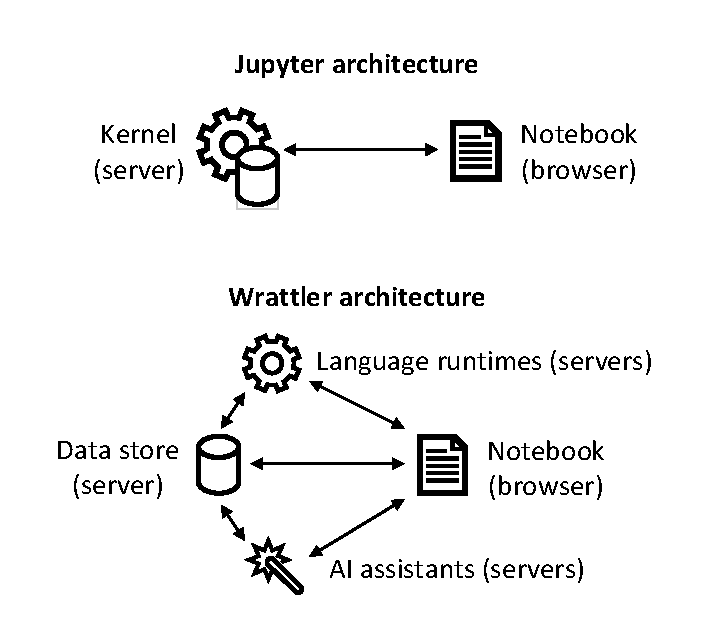
\includegraphics[scale=0.6]{diagram.pdf}
\vspace{-1em}
\caption{\small{In notebook systems such as Jupyter, state and execution is managed by a kernel. In
  Wrattler, those functions are separated and enriched with AI assistants.}}
\label{fig:arch}
\vspace{-1em}
\end{figure}

\section{Wrattler components}

Wrattler consists of a notebook user interface running in the web browser, which communicates with 
a number of server-side components including language runtimes, the data store and AI assistants. 
In this section, we discuss the components in more detail, starting with the dependency graph
that is maintained on the client-side, by the web browser.

\subsection{Dependency graph}

When opening a notebook, Wrattler parses the source of the notebook (consisting of text cells and 
code cells) and constructs a dependency graph, which serves as a runtime representation of the
notebook. 

The structure is ilustrated in Figure~\ref{fig:deps}. Top-level nodes (squares) represent
individual notebook cells. Code (circles) is represented either as a single node (R, Python) or as 
a sub-graph with node for each operation (DSLs understood by Wrattler). Any node of a cell can 
depend on a data frame (hexagons) exported by an earlier cell. 
When code in a cell changes, Wrattler updates the dependency graph, keeping existing
nodes for entities that were unaffected by the change. 

The dependency graph enables several features that are difficult for most notebook systems:
%
\begin{itemize}
\item[--] When code changes, Wrattler only needs to recompute small part of the graph.
  This makes it possible to provide live previews, especially for simple data analytical DSLs.
\vspace{-0.85em}
\item[--] Refactoring can extract parts of the notebook that
  are needed to compute a specified output.
\vspace{0.25em}
\item[--] Refactoring can translate nodes of an analytical DSLs (generated by an AI assistant) into R or Python.
\vspace{0.25em}
\item[--] The graph can be used for other analyses and refactorings, such as provenance tracking
  or code cleanup.
\end{itemize}

\subsection{Data store}

The data store provides a way for persistently stroing data and enables communication between 
individual Wrattler components. Data store keeps external data files imported into Wrattler,
as well as computed data frames (and, potentially, other data structures). It is immutable 
and keeps past versions of data to allow efficient state rollback. For persistency and versioning, 
data store also serializes and stores multiple versions of the dependency graph.

The data store supports a mechanism for annotating data frames with additional semantic information, such as:
%
\begin{itemize}
\item[--] Columns can be annotated with (and stored as) primitive data type such as date or floating-point number.
\vspace{0.25em}
\item[--] Columns (or a combination) can be annotated with semantic annotation such as geo-location or and address.
\vspace{-0.85em}
\item[--] Columns, rows and cells of the data frame can be annotated with other metadata such as provenance.
\end{itemize}

\subsection{Language runtimes}

Language runtimes are responsible for evaluating code and assisting with code analysis during
the construction of dependency graph. They can run as server-side components (e.g.~for R and Python) 
or as client-side components (for JavaScript and small analytical DSLs used by AI assistants). 
Unlike Jupyter kernels, a language runtime is stateless. It reads data from and writes data to
the data store. (Using a cache for efficiency.)


\begin{figure}
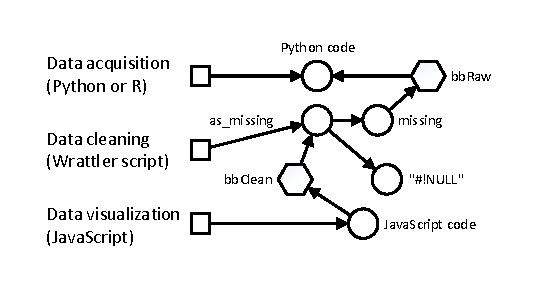
\includegraphics[scale=1,trim=0.5cm 0.5cm 0.5cm 0.5cm]{graph.pdf}
\vspace{-0.5em}
\caption{\small{Sample dependency graph. Data acquisiton and analysis are represented as 
opaque R/Python code cells. Data cleaning is written in a domain-specific langauge understood by
Wrattler and represented by multiple cells. Latter two cells depend on data frames exported by
earlier cells.}}
\label{fig:deps}
\vspace{-0.5em}
\end{figure}

\subsection{AI assistants}

The Wrattler architecture enables integration of AI assistants in a number of ways. First, AI
assistants have access to the data store (and the dependency graph) and can use those to provide
guidance about both data and code. Second, Wrattler includes an extensible framework for defining
domain-specific languages (DSLs) that can describe, for example, data extraction, cleaning, transofrmation or 
visualization. An AI assistant can work in two ways:
%
\begin{itemize}
\item[--] When invoked, the assistant creates a new frame in the data store with additional
  information, e.g. probabilistic type inference (ptype) will annotate columns (and possibly
  also cells) with their probabilistic types.
\vspace{0.25em}
\item[--] The assistant defines a DSL for the task at hand. When invoked from a notebook,
  it guides the user in creating a script in the DSL that performs the required operation
  (such as extracting data or reformatting a data frame).
\end{itemize}
%
The second case is illustrated in Figure~\ref{fig:arch}. An AI assistant reads data from the data
store and returns suggestions in a small DSL to the notebook, which the user can review 
(using a live preview mechanism) and accept. For example, an AI
assistant based on datadiff can suggest the following script (written using the Wrattler DSL
framework):
%
\begin{equation*}
\begin{array}{l}
\ident{datadiff(broadband2014, broadband2015)}\\
\quad.\ident{drop\_column}(\str{WT\_national})\\
\quad.\ident{drop\_column}(\str{WT\_ISP})\\
\quad.\ident{recode\_column}(\str{URBAN}, [\num{1}, \num{2}], [\str{Urban},\str{Rural}])
\end{array}  
\end{equation*}
%
The script specifies that two columns should be dropped from the badly structured data frame and
one column needs to be recoded (turning $\num{1}$ and $\num{2}$ into strings
\strf{Urban} and \strf{Rural}).

The above script is constructed interactively. When the user types the first line and types
``.'' the datadiff assistant offers the most likely patches and the user can choose. While
choosing, a preview of the result is computed on-the-fly, giving the user an immediate feedback.
Finally, the script is represented in a fine-grained way (second cell in Figure~\ref{fig:deps}).
Once it is interactively constructed, it can be translated to multiple supported languages
such as R, Python or JavaScript.
\end{document}
